\documentclass[11pt]{article}

\usepackage{amsmath}
\usepackage{textcomp}
\usepackage[top=0.8in, bottom=0.8in, left=0.8in, right=0.8in]{geometry}
\usepackage{listings}
\usepackage{graphicx}
\usepackage{subcaption}


% Add other packages here %


% Put your group number and names in the author field %
\title{\bf Excercise 3\\ Implementing a deliberative Agent}
\author{Group 24: Benvenuti Eloi Jean, Timoth\'ee-Florian S\'ebastien Bronner}


% N.B.: The report should not be longer than 3 pages %


\begin{document}
\maketitle

\section{Model Description}
Here's how we modelised the problem.

\subsection{Intermediate States}
% Describe the state representation %
A state is defined by:

\begin{itemize}
	\item The city in which the vehicle is.
	\item The tasks currently carried by the vehicle.
	\item The tasks currently available for pickup.
\end{itemize}
\subsection{Goal State}
% Describe the goal state %
A goal state is reached when the vehicle isn't carrying any task and there are no task available for pickup.

\subsection{Actions}
% Describe the possible actions/transitions in your model %
An action consist of either going to a city and picking up a task or going to a city and delivering a task.

\section{Implementation}

\subsection{BFS}
% Details of the BFS implementation %
\paragraph{State class} The State.java contains the class representing the state. In this class we store the city the vehicle is currently in, a set of all the tasks carried by the vehicle and a set of all the available tasks in the world. We also store the list of action taken to reach that state, the cost of the state and the total weight carried by the vehicle.

%Talk about the fact that this makes us not respect our definition of task and why we did this (find the best solution

\subsection{A*}
% Details of the A* implementation %

%Mention the hashmap of <state,cost> and how this implement our state representation.

\subsection{Heuristic Function}
% Details of the heuristic functions: main idea, optimality, admissibility %

%Speak about how we first discriminated more against state that had more tasks not yet picked up and that it led to poorer performances.


\section{Results}

\subsection{Experiment 1: BFS and A* Comparison}
% Compare the two algorithms in terms of: optimality, efficiency, limitations %
% Report the number of tasks for which you can build a plan in less than one minute %
We compare here the two algorithms BFS and A*. 

\subsubsection{Setting}
% Describe the settings of your experiment: topology, task configuration, etc. %
The two algorithms will be compared using the topology Switzerland, the politique of short distance. At first the number of task each algorithm is able to handle in less than one minute will be determinated (running on a Lenovo Thinkpas W540 laptop).

Then the algorithms will be tested with different starting state to see if one consistantly perform as least as well as the other and sometimes better. 10 tests with the highest possible number of tasks (5) will be performed. 
\subsubsection{Observations}
% Describe the experimental results and the conclusions you inferred from these results %
The limite of tasks for which a plan can be made in less than a minute is the following:
\begin{itemize}
  \item BFS: 5 tasks
  \item A*: 7 tasks
\end{itemize}
It should be noted that after this limite the computation fail on both algorithms. For the BFS a OutOfMemory occurs and a time out for the A*.

Both algorithms arrive each time at the same cost, which seems to indicate that both find the optimal solution. Moreover, for the 10 tests they have always outperform the random algoritm. Therefore A* seems preferable to BFS as it will be able to be implemented for larger problems, for the same final result.

\subsection{Experiment 2: Multi-agent Experiments}
% Observations in multi-agent experiments %
The agents compute the plan with all the tasks that he can see, the task in the world and the tasks that they carry. Therefore, should another agent pick up a task, the whole plan must be recomputed.  
\subsubsection{Setting}
% Describe the settings of your experiment: topology, task configuration, etc. %
The topology is again Switzerland with 5 tasks. Now, the comparision will be made on the graph of the reward per km, see Figures \ref{img:multipleAgent}. There is now 1 to 3 agents in the world. 

\subsubsection{Observations}
% Describe the experimental results and the conclusions you inferred from these results %
Figures \ref{img:multipleAgent} show the result for 1, 2 or 3 agents in the world. The result doesn't change depending on the fact that the agent use BFS or A*, only of the starting position (for a given starting state).
This figures show the inneficiency to have more than one agent. Firstly, the mean reward per Km for respectively 2 and 3 agents is about 60\% and 50\% of the reward for only one agent. Secondly, some agent will move without being able to pickup a task because another would have been first. They will only stop when no more task will be available.
\begin{figure}
  \begin{subfigure}[b]{0.3\textwidth}
    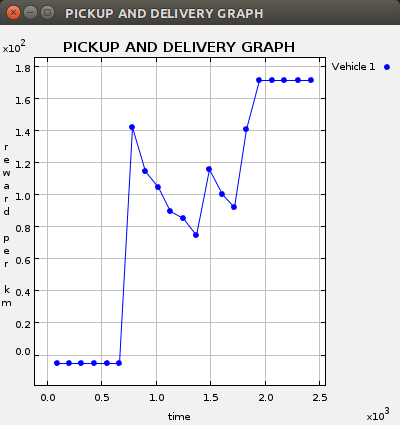
\includegraphics[width=\textwidth]{1agent.png}
    \caption{Single agent}
    \label{img:1agent}
  \end{subfigure}
  \begin{subfigure}[b]{0.3\textwidth}
    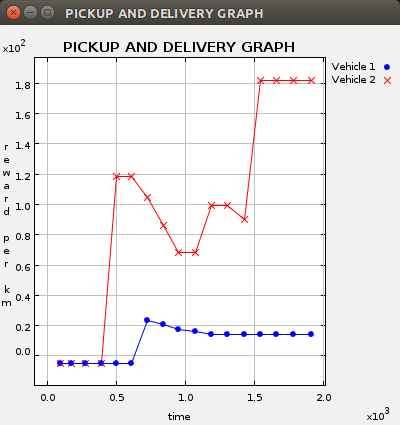
\includegraphics[width=\textwidth]{2agentsBFSASTAR.png}
    \caption{2 agents}
    \label{img:2agents}
  \end{subfigure}
  \begin{subfigure}[b]{0.3\textwidth}
    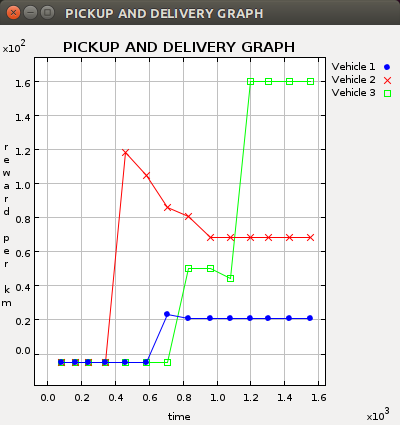
\includegraphics[width=\textwidth]{3agentsBBA.png}
    \caption{3 agents}
    \label{img:3agents}
  \end{subfigure}
  \caption{Comportment of the agents depending on their number in the world.}
  \label{img:multipleAgent}
\end{figure}
\end{document}
